Tra le due componenti in cui si articola il progetto, la prima sviluppata è stata la componente \emph{client}. Questa parte consiste sostanzialmente di una applicazione per dispositivi \emph{smartphone} Android, completamente riscritta a partire da alcuni sviluppi precedenti per poter assolvere alle nuove funzioni specifiche di \emph{PathS}. Le attività di studio e implementazione sono state svolte da Stefano Tombolini e documentate nella relativa tesi di Laurea \cite{tesitombolini}. Si riassumono nel capitolo seguente i requisiti che sono stati identificati e i criteri principali che hanno determinato lo sviluppo del software così da fornire una visione più completa dello sviluppo del progetto. 

\section{Requisiti}
Il client mobile \emph{PathS} presenta tutte le caratteristiche di una applicazione sviluppata secondo il paradigma \emph{Web\textsuperscript{2}}. 
Le funzioni principali che deve svolgere possono essere riassunte in:
\begin{itemize}
\item raccogliere dei valori riguardante l'ambiente circostante tramite i sensore di luminosità e microfono;
\item tenere traccia degli spostamenti effettuati e abbinarli ai relativi campioni;
\item offrire le indicazioni di percorso secondo la destinazione e le modalità richieste dall'utente;
\item cercare di coinvolgere il più possibile l'utente incentivando l'uso dell'applicazione.
\end{itemize}

Alcuni di questi requisiti possono essere identificati come \emph{funzionali} e sono indispensabili per gli scopi generali del progetto. Le operazioni di campionamento tramite i sensori ambientali e il tracciamento della posizione tramite GPS sono gli elementi fondamentali richiesti per poter disporre dei dati necessari alle successive elaborazioni. Tuttavia nessun utente finale sarebbe motivato nell'eseguire queste operazioni se l'applicazione non fornisse una qualche altra utilità. Un gruppo di utenti volontari può essere selezionato per alcune campagne di raccolta, tuttavia per motivare un utilizzatore occasionale era necessario adottare altre strategie. 
Per questo sono stati identificati gli altri due requisiti, così da motivare l'utilizzo dell'applicazione stessa. Si è pensato che fornendo direttamente il servizio di \emph{routing} dallo smartphone, si potevano sfruttare i risultati del servizio ma contemporaneamente contribuire allo stesso raccogliendo ulteriori informazioni durante il percorso. Per rendere ottimali i dati raccolti durante l'uso, era inoltre necessario ideare uno stratagemma affinchè il dispositivo fosse in una condizione ideale per il campionamento. La soluzione è venuta dalla proposta di adottare delle funzioni di \emph{Augmented Reality} (Realtà Aumentata). In questo modo non solo si sarebbe ottenuto un maggiore coinvolgimento dell'utente finale, ma inconsapevolmente l'utilizzatore stesso avrebbe mantenuto lo \emph{smartphone} fuori dalla tasca in condizioni perfette per le misurazioni tramite i sensori.
Seguendo queste indicazioni quindi, si è strutturata una applicazione \emph{Android} composta principalmente di 3 moduli:
\begin{itemize}

\begin{figure}[ht]
  \centering
  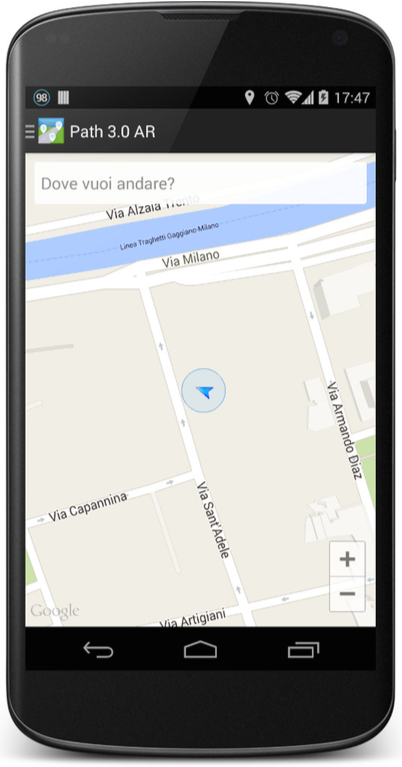
\includegraphics[width=.5\textwidth]{app-mappa}
  \caption{\footnotesize{Modalità \emph{Mappa} dell'applicazione mobile PathS.}}
  \label{fig:app-mappa}
\end{figure}

\item \textbf{Mappa}: E' la schermata con la quale l'utente può selezionare una destinazione e visualizzare il percorso suggerito. In questa sezione l'applicazione comunica con i servizi Google per la selezione dei luoghi e la ricerca della destinazione, mentre interroga la componente \emph{server} di \emph{PathS} per richiedere i percorsi da suggerire. Il risultato è visualizzato in una vista a cartina stile Google Maps.

\begin{figure}[ht]
  \centering
  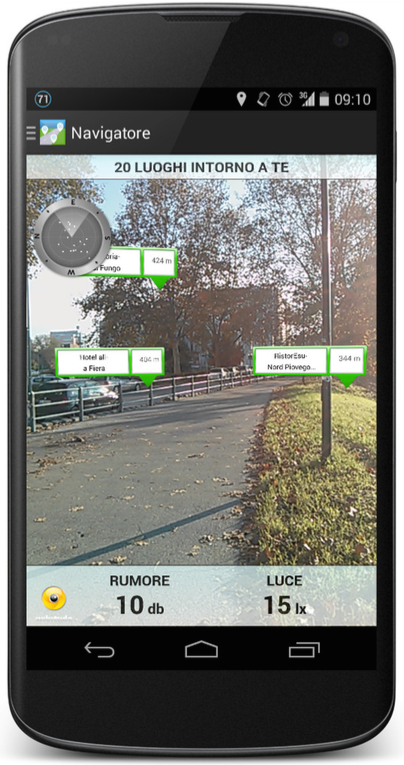
\includegraphics[width=.5\textwidth]{app-navigatore}
  \caption{\footnotesize{Modalità \emph{Navigatore} dell'applicazione mobile PathS.}}
  \label{fig:app-navigatore}
\end{figure}

\item \textbf{Navigatore}: E' la modalità con la quale si guida l'utente durante il percorso pedonale: si forniscono le indicazioni di svolta ed altre informazioni aggiuntive presentandole in realtà aumentata. L'utente può quindi mantenere il dispositivo in posizione verticale inquadrando l'orizzonte con la fotocamera e visualizzare in modo sovrapposto le informazioni di cui necessita. Durante questa modalità sono eseguiti in \emph{background} i campionamenti di rumorosità e luminosità che saranno successivamente inviati al server.
\item \textbf{Impostazioni}: In questa parte dell'applicazione è possibile configurare alcuni parametri di funzionamento e di visualizzazione.
\end{itemize} 

I tre moduli consentono all'applicazione di svolgere tutte le funzioni identificate dai requisiti.

\section{Tecnologie}
Considerando gli sviluppi precedenti e la disponibilità di dispositivi, la piattaforma scelta per lo sviluppo del client è stato il sistema \emph{Android}. Questo sistema operativo è ormai largamente diffuso sia nei dispositivi tablet che smartphone anche di fascia economica, risultando un ottimo candidato per poter raggiungere una larga base di utenza. Le caratteristiche \emph{Open Source} del sistema hanno reso inoltre più agevoli le modalità di sviluppo e installazione del software piuttosto che le alternative proprietarie ad esempio \emph{iOS}.
Le tecnologia principale con cui è stata realizzata l'applicazione è stata quindi l'\emph{Android Software Development Kit (SDK)}. Questo framework mette a disposizione tutte le librerie e i \emph{tool} necessari allo sviluppo del modulo client. Oltre alle funzioni di interfacciamento grafico e logica applicativa, l'\emph{SDK} consente anche di sfruttare in modo agevolato i sensori hardware del dispostivo (luminosità e microfono) nonchè il sotto-sistema \emph{GPS}, tutte funzioni particolarmente critiche per la riuscita del progetto.
Un'altra libreria fondamentale utilizzata nello sviluppo dell'applicazione mobile \emph{PathS} è stata \emph{Wikitude}. Questa libreria è stata selezionata tra altre analoghe, e il suo ruolo è stato quello di offrire le funzionalità di realtà aumenate richieste dalla soluzione. 
Per ulteriori dettagli riguardanti la selezione degli strumenti e l'implementazione dell'applicazione client si rimanda alla tesi specifica \cite{tesitombolini}.

\section{Stato attuale}
In generale l'applicazione \emph{client} presenta tutte le carateristiche indispensabili dal punto di vista funzionale per consentire lo sviluppo della controparte \emph{server}.

L'operazione di trasmissione dei campioni al server viene eseguita correttamente, così come l'interrogazione dei risultati disponibili e la presentazione degli stessi all'utente in modalità mappa e navigazione \emph{turn by turn}.

Tuttavia ci sono alcune aree importanti in cui una revisione consentirebbe un miglioramento dei dati forniti alla componente \emph{server} e un utilizzo più pratico dell'applicazione. 
I punti di intervento proposti si riassumono in:
\begin{itemize}
\item Correzione della scala dei valori raccolti e normalizzazione degli stessi, in particolare per quanto riguardo la luminosità. Nei test eseguiti molti valori raggiungono il $100\%$, presentando pochi casi con valori intermedi nonostante le diverse situazioni reali di applicazione. Questa imprecisione si ripercuote sull'intero sistema e i servizi forniti, influenzando direttamente i risultati finali.
\item Miglioramento delle modalità con cui si comunica all'utente la trasmissione dei dati al server, rendendo esplicito il momento in cui tale comunicazione avviene ed eventuali malfunzionamenti (rete non presente, connessione fallita, etc).
\item Miglioramento della responsività della app, in particolare nell'accesso al modulo di navigazione che spesso non è \emph{smooth} in particolare in dispositivi non performanti. In generale i rallentamenti nel feedback e il funzionamento scattoso peggiorano l'esperienza utente e disincentivano l'utilizzo della app.
\item Verificare il consumo di risorse che si verifica durante l'esecuzione di tutte le operazioni in \emph{background}, valutando una ottimizzazione delle stesse. In molti casi si è verificato un consumo abbondante della carica batteria e talvolta anche un surriscaldamento del dispositivo.
\end{itemize}
Al netto degli spunti di possibile miglioramento, lo stato attuale dell'applicazione mobile ha comunque consentito e supportato lo sviluppo della componente server e quindi dell'intera soluzione \emph{PathS}. Le versioni aggiornate dell'applicazione possono essere scaricate dal sito del progetto \cite{paths-graphs}.
